\documentclass{ximera}
\input{../preamble}
\addPrintStyle{..}

\begin{document}
	\author{Zomercursus KU Leuven}
	\xmtitle{Opmerkingen}{nog ergens te integreren}

    % nog ergens toe te voegen ..?
    
    \begin{remark} \nl
    \begin{itemize}
        \item Een complex getal kan per definitie op een unieke manier geschreven worden als $a+bi$, met $a,b\in\R$. Dus $1, i, 1+i, 1+3i$ zijn allemaal complexe getallen die we niet eenvoudiger kunnen schrijven. Maar $2i+3+i, i(1+i)$ en $(1+i)(1-i)$ zijn complexe getallen die we wel eenvoudiger kunnen schrijven als $2i+3+i=3+3i, \quad i(1+i)=i+i^2 =-1+i,\quad  (1+i)(1-i) = 1 - i^2 = 1+1 =2$.
        
        \item Als je twee complexe getallen kan optellen, is het ook eenvoudig om ze van elkaar af te trekken: $(a_1+b_1i)-(a_2+b_2i) = (a_1-a_2)+(b_1-b_2)i$. Je kan twee complexe getallen ook \textit{delen} door elkaar, dit wordt later uitgelegd.
    %    maar dat is wat complexer \xmopje{(pun intended)}. Je kan er zelf eens over nadenken, maar we geven hier geen formule voor de deling van complexe getallen. Delen zal verder een eenvoudige toepassing blijken te zijn van de \textit{inverse} van een complex getal.
        
        \item Ingenieurs gebruiken meestal de letter $j$ in plaats van $i$, onder meer om verwarring te voorkomen met de elektrische stroom $i$. Dan geldt dus $j^2=-1$, en $z=a+bj\in\C$.
        
        \item 
        Men kan aantonen dat de verzameling $\C$ \textbf{niet totaal kan geordend worden} zoals $\Q$ of $\R$. Hiermee wordt bedoeld dat het niet mogelijk is om een definitie te vinden voor $a+bi <c+di$ die zou voldoen aan dezelfde eigenschappen als de ongelijkheid $<$ in $\R$ of $\Q$. Je kan van twee complexe getallen dus niet zeggen welk "{}het kleinste{}" is.
    %	 (Het begrip \textit{modulus} zal verder toch een soort 'grootte' introduceren, maar complexe getallen kunnen 'dezelfde grootte' hebben zonder aan elkaar 'gelijk' te zijn. Die 'grootte' gedraagt zich dus toch erg anders dan de 'orde' op $\R$.)   )
        \\ 
        In het bijzonder heeft het geen betekenis om te vragen of $2+3i$ \textit{positief} of \textit{negatief} is. 
        Zo kan je ook niet zeggen dat $1+i$ \textit{positief} is en $-1-i$ \textit{ negatief}, maar wel dat ze elkaars \textit{tegengestelde} zijn. Hetzelfde geldt zelfs voor $i$: het heeft geen betekenis om te beweren dat $i$ positief is, en $-i$ negatief. Het heeft wel betekenis om te zeggen dat $i$ en $-i$ elkaars tegengestelde zijn.
        
    %    \item Voor het reëel en imaginair deel van $z=a+bi$ worden soms andere notaties gebruikt: \\ $a=\Re(z)=\text{Re}(z)=\text{Re}(a+bi)$, en  $b= \Im(z)=\text{Im}(z)=\text{Im}(a+bi)$.
    \end{itemize}
    \end{remark}
    


\begin{exercise}
    Schets in het complexe vlak de gebieden omschreven door volgende vergelijkingen:
    \begin{question} 
        $\text{Im}(z) \leq 0$
        \begin{oplossing} Als $z=a+bi$, dan betekent Im$(z) \leq 0$ dat $b \leq 0$ en dat geeft het  halfvlak onder de $x$-as:
            \begin{image}[0.2\textwidth]
                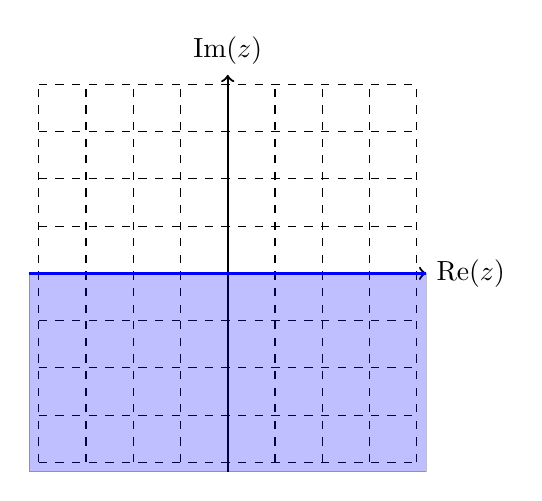
\begin{tikzpicture}[scale=0.6]
                \draw[dashed] (-4, -4) grid (4, 4);
                
                \draw[->, thick] (-4.2, 0) -- (4.2, 0) node[right] {Re$(z)$};
                \draw[->, thick] (0, -4.2) -- (0, 4.2) node[above] {Im$(z)$};
                
                \draw[fill=blue, opacity=0.25] (-4.2,-4.2) rectangle (4.2,0);
                
                % randen toevoegen voor duidelijkheid 
                \draw[blue, very thick] (-4.2,0) -- (4.2,0);
                \end{tikzpicture}
            \end{image}
			
        \end{oplossing}
    \end{question}
    
    \begin{question} 
        $0 \leq \text{Re}(z) \leq 2$
        \begin{oplossing} Deze ongelijkheden bepalen een \textit{verticale} strook, aangezien het reële deel van het complex getal in een interval moet liggen. De randen van de strook behoren tot het geschetste domein.
            
            \begin{image}[0.2\textwidth]
                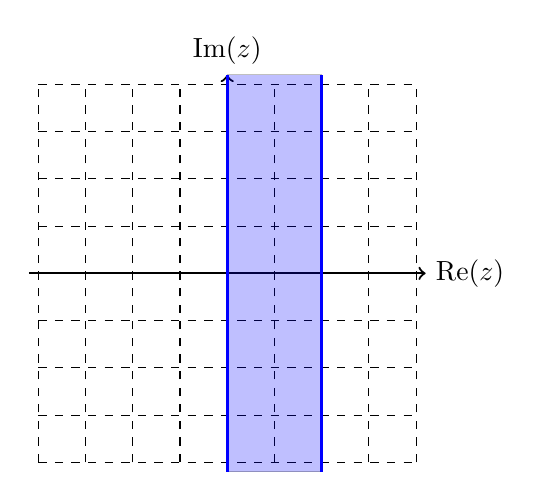
\begin{tikzpicture}[scale=0.6]
                \draw[dashed] (-4, -4) grid (4, 4);
                
                \draw[->, thick] (-4.2, 0) -- (4.2, 0) node[right] {Re$(z)$};
                \draw[->, thick] (0, -4.2) -- (0, 4.2) node[above] {Im$(z)$};
                
                \draw[fill=blue, opacity=0.25] (0,4.2) rectangle (2, -4.2);
                
                % randen toevoegen voor duidelijkheid 
                \draw[blue, very thick] (0, -4.2) -- (0, 4.2);
                \draw[blue, very thick] (2, -4.2) -- (2, 4.2);
                \end{tikzpicture}
            \end{image}
        \end{oplossing}            
    \end{question}        
    \end{exercise}


\end{document}

